\documentclass[a4paper,11pt]{jsarticle}


% 数式
\usepackage{amsmath,amsfonts}
\usepackage{bm}
% 画像
\usepackage[dvipdfmx]{graphicx}


\begin{document}

\title{Phase transition encoded in neural network}
\author{須賀勇貴}
\date{最終更新日:\today}
\maketitle
これは,柏,菊池,富谷先生による論文"Phase transition encoded in neural network"を日本語でまとめたものである.\par

\subsection*{Abstract}
相転移検出を目的としたニューラルネットワークの一側面について論じる.そのために,まず温度でラベル付けされたイジング模型とポッツ模型の配位データで温度を測定させるようにニューラルネットワークを構築して学習させる.ここで,私たちは,機械に配位が秩序相にあるか無秩序相にあるかは明示的に与えていないことに注意してほしい.にもかかわらず,学習したニューラルネットワークはパラメータ(重みをバイアス)から臨界温度を特定することができる.私たちは,温度教師付きニューラルネットワークがどのような量を学習するかに注目することで,相転移の情報をどのように捉えるか理解しようと試みる.私たちの詳細な分析により,機械は学習の程度に応じて異なる物理量を学習していることが明らかになった.この研究の主な観察は,学習済みニューラルネットワークの重みが温度に加えて,相転移の情報をどのように持つかということである.

\section{はじめに}
物質の相を探索することは,基礎となる微視的な物理システムの赤外線構造を明らかにするための最も重要な課題である.これらの相は,理論の持つ対称性に基づいて分類される.いくつかの異なる相を含む理論では,相転移はそれらの境界で発生する.それらのうち,二次相転移の性質は次元の数によってのみ決定され,微視的な詳細とは独立した大域的対称性の基礎理論,つまり,普遍性クラスによって分類される.しかしながら,実際のところ,微視的な理論データに基づいて位相を解析したり,相転移を検出したりすることは一般的に難しい課題である.なぜなら,それらの問題を正確に解決すること,もしくは対応する赤外理論を特定することが難しいためである.したがって,これらの問題を解明するためには,数値的なアプローチが大量に取り組まれてきた.明白で主要な障害は,自由度の数が増加するにつれて,数値解析がますます困難になることである.\par
機械学習はコンピュータサイエンスの分野で急速に発展し,パターン認識,画像処理などで顕著な成功を収めてきた.最近では,機械学習が物理学のさまざまな分野でも適用されていることが目撃されている.相転移の検出は,機械学習が新たな進展を遂げる可能性がある興味深い例の一つであり,すでにスピンシステムなどの単純なモデルでいくつかアプローチが提案され,試験されている.これらの研究は,教師あり学習では[3-18],教師なし学習では[19-24]などで行われている.ここでは,入力データはニューラルネットワークやその学習プロセスとは独立して準備されてる.例えば,モンテカルロシミュレーションや興味を持つ物理系に基づく実験データが,必要な入力データを提供する.\par
物理系の相境界を検出する一つのアプローチは,教師ありバイナリ分類である.ここでは,ニューラルネットワークが学習され,それが秩序だったり無秩序だったりする相を区別できるようになる.実際に,このアプローチは生成データからいくつかのモデルの相転移を合理的に検出する[3].最近では,潜在変数と物理量との間の暗黙のつながりに関する研究が広く行われ,機械学習技術のブラックボックス性を取り除く究極の目標に向けて進展が見られている[3, 12, 15, 18].また,物理的な洞察に基づく特徴エンジニアリングの支援を受けて,トポロジカル相転移やBKT相転移などの非標準的な相転移も検出に成功した[10, 12, 14, 16, 25, 26].\par
別の興味深いアプローチが[4]で提案され,相転移を検出するために,秩序パラメータの情報が学習の結果としてニューラルネットワークの重みにエンコードされていると仮定している.彼らは教師あり機械学習を用いて,2次元のIsing模型の臨界温度を特定しようとした.全結合ニューラルネットワークと畳み込みニューラルネットワークは,入力のスピン構造の目標温度を正確に予測できるように学習された.驚くべきことに,学習中に相転移に関する直接の情報を与えていないにもかかわらず,彼らは重みから相転移温度を抽出することに成功した.これは,ネットワークが温度の教師付き学習の過程で相転移を自発的に捉え,機械パラメータにエンコードしていることを意味している.しかし,その結果の基本的なメカニズムは未解決のままである.\par
この記事の目的は,この相転移検出のメカニズムを理解することである.このアプローチが捉えるものを理解することは,それを他の未知のシステムに適用しようとする際に役立つ.異なる物理的メカニズムによって引き起こされる場合,例えば準長距離秩序(BKT転移)や位相など、正確に相転移を検出できない可能性があるからである.実際,この方法は,ニューラルネットワークの学習方法によって異なる物理量,つまり入力配位の特徴を捉えることが分かる.アイデアを説明するために,温度予測の本質を具現化した簡略化されたニューラルネットワークの構造に注目する.

\section{臨界温度予測}
2次元イジング模型を考える.ハミルトニアンは
\begin{equation*}
  H(\bm{\sigma}) = - J \sum_{\langle i,j \rangle} \sigma_i \sigma_j
\end{equation*}
ここで,$J$は結合定数,$\sigma_i \in \{ -1, 1 \}$は,サイズが$L \times L$の正方格子のサイトに存在するスピンの自由度(スピン変数)で,周期的境界条件が課されている.和は最近接に対するサイトにわたる.結合定数をボルツマン重みに吸収させて,$e^{-KH}/Z, \ \ K = \beta J$とすることで,ハミルトニアンを次のように再定義する.
\begin{equation}
  H(\bm{\sigma}) = - \sum_{\langle i,j \rangle} \sigma_i \sigma_j
\end{equation}
ここで,$Z = \sum_{\bm{\sigma}}e^{-KH(\bm{\sigma})}$は分配関数である.\par
私たちは,その2次相転移に関連する臨界温度を検出しようと試みている.しかしながら,最初は,教師あり順伝播ニューラルネットワークを用いて温度測定器を構築することを行う.その後,学習されたニューラルネットワークの重みとバイアスを調べ,2次元イジング模型と3状態のポッツ模型の臨界温度を特定しようと試みる.\par
メトロポリス・ヘイスティングス法を用いて,各温度で2000個のイジングスピン配位を生成する.これらは,20の目標温度と一緒にニューラルネットワークに供給される.私たちは,TENSORFLOWをバックエンドに使用したKERASパッケージを用いて,全結合ニューラルネットワークと畳み込みニューラルネットワークの2種類のアーキテクチャを実装した.\par
全結合ニューラルネットワーク:
\begin{equation}
  \left[
    \begin{aligned}
       & \mathcal{I} = \left\{ \{ \sigma_i \} \Big| \ \text{Ising configs on} \ L \times L \ \text{lattice.} \right\} \\
       & \downarrow
      \begin{cases}
        \text{Fully-connected (Dense) layer} \\
        \text{Softmax activation}
      \end{cases}                                                                            \\
       & x_a \in [0,1]^{N_h} \ \text{: hidden units}                                                                  \\
       & \downarrow
      \begin{cases}
        \text{Fully-connected (Dense) layer} \\
        \text{Softmax activation}
      \end{cases}                                                                            \\
       & y_K \in [0,1]^{N_o} \ \text{: output}
    \end{aligned}
    \right]
\end{equation}

入力の自由度は$\{ \sigma_i \} \ (i=1,2,\dots,L \times L)$で,イジングモデルの場合スピンに対応する.隠れ層のユニット$x_a \ (a=1,2,\dots,N_b)$は
\begin{equation}
  x_a = \text{softmax}(w_{ai}^{(1)}\sigma_i + b_a^{(1)})
  \equiv \frac{e^{w_{ai}^{(1)}\sigma_i + b_a^{(1)}}}{\sum_a e^{w_{ai}^{(1)}\sigma_i + b_a^{(1)}}}
\end{equation}
ここで,アインシュタインの縮約記法を使用していることに注意.2つ目の層は,重み$w_{\alpha a}^{(2)}$とバイアス$b_{\alpha}^{(2)}$に置き換えたものである.最終層の変数$y_K \ (K=1,2,\dots,N_o)$は隠れ層と同じ形をとる
\begin{equation}
  y_k = \text{softmax}(w_{ai}^{(2)}\sigma_i + b_a^{(2)})
\end{equation}
出力$\{ y_K \}$に基づいて,入力配位の温度は
\begin{equation}
  K^{\text{output}} = \underset{K} {\operatorname{argmax}} (y_K)
\end{equation}
で決定される.つまり,温度$\alpha$は確率分布$y_K$の中から最も値が高い成分が採用されるということである.学習は,Adamという最適化手法を用いて,交差エントロピー
\begin{equation}
  E(y_K,\bm{1}_{K=K_i^{\text{target}}}) = - \frac{1}{N_o}\sum_i \bm{1}_{K=K_i^{\text{target}}} \ln{y_k}
\end{equation}
という誤差関数を最小することによって実装した.ここで,$i$ は入力配位のラベルを示す.インジケーター関数は次のように定義される.\par
\begin{equation}
  \bm{1}_{K=K_i^{\text{target}}} =
  \begin{cases}
    1 & (K=K_i^{\text{target}}) \\
    0 & (\text{otherwize})
  \end{cases}
\end{equation}

畳み込みニューラルネットワークは3つの畳み込み層と最後の全結合層からなる構成をしており,式(\ref{conv model})である.これについての詳細はセクション3.2で説明する.\par
配位生成から相転移検出までの手順を以下に示す.
\begin{enumerate}
  \item マルコフ連鎖モンテカルロ法より,配位を生成:
  \item ニューラルネットワークを温度計として学習する.入力はスピン配位,出力は予測温度.
  \item ニューラルネットワークに現れる学習済みの重みとバイアスを分析する.マシンパラメーターに相転移の情報がどのように含まれるかについて説明する.
\end{enumerate}

\subsection{2次元イジング模型}
\begin{figure}[hb]
  \begin{center}
    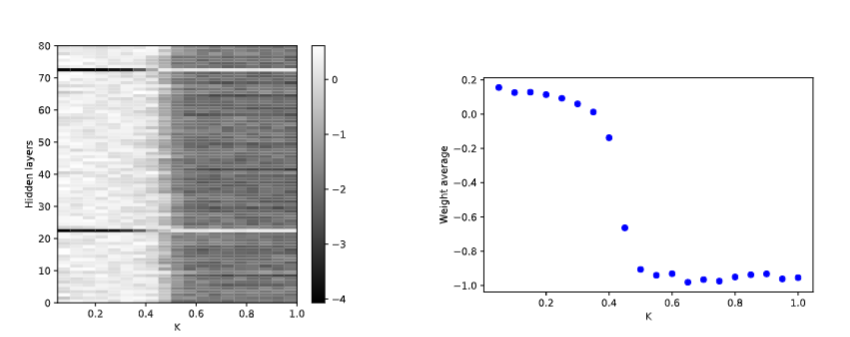
\includegraphics[height=5cm]{image/Figure1.png}
    \caption{2次元イジング模型における学習後の全結合層での重みの値とそれらを平均した値.横軸はそれぞれ入力配位の温度$K$を表している.縦軸は左の図はニューラルネットワークの隠れ層につながるエッジにおける重みの値に対応し,右の図はその重みの値を$K$での平均をとったものである.重みの平均の値は,厳密な臨界温度$K_{\text{c}}^{\text{exact}}\simeq 0.4407$付近で大きく変化していることが見て取れる.}
  \end{center}
\end{figure}
最初に,[4] (田中さんと富谷さんの論文)で既に研究されている2D Ising模型を見ていく.このモデルは,100の目標温度で調査され,その重みは秩序変数のように振る舞い,すなわち自発的な磁化を示す.私たちの主な目的は臨界温度を定量的に推定することではなく,そのメカニズムを理解することなので,目標温度の数を20に減少させる.具体的には,$K = 0.05, 0.1, 0.15, \dots, 1.0$のような値である.ニューラルネットワークより教師あり機械学習を行った.

図1
2D Ising模型の場合,全結合層の重みおよびそれらの学習後の平均について説明する.横軸は入力配位の温度Kを表し,左のパネルの縦軸はニューラルネットワークの隠れユニットに接続された成分に対応している.右のパネルの縦軸は,各Kに対する重みの平均を示している.重みの平均値は,正確な臨界温度$K_e^{\text{exact}} \approx 0.4407$の周りで著しく変化している.


格子サイズは$L = 16$であり,隠れユニットの数は$N_h = 80$,そして$N_o = 20$はそれぞれ20の目標温度に対応している.臨界温度は正確に知られており,$K_c^{\text{exact}} = \frac{1}{2}\ln{\sqrt{2}+1} \approx 0.4407$である.学習後の2層目の重みが図1である([4]より).臨界温度は重みの和を$c_1 \tanh{[c_2(K-K_c)]}$でフィッティングしてパラメータ$c_1,c_2,c_3$を導くことで予想する.実験では格子サイズ$L=8,16,32$で行った.実際,最終的な重みの平均は秩序変数のように振る舞うようです(図1の右パネル).次のセクションで重みの詳細な構造について議論します.


\subsection{2次元3状態ポッツ模型}
\begin{figure}[hb]
  \begin{center}
    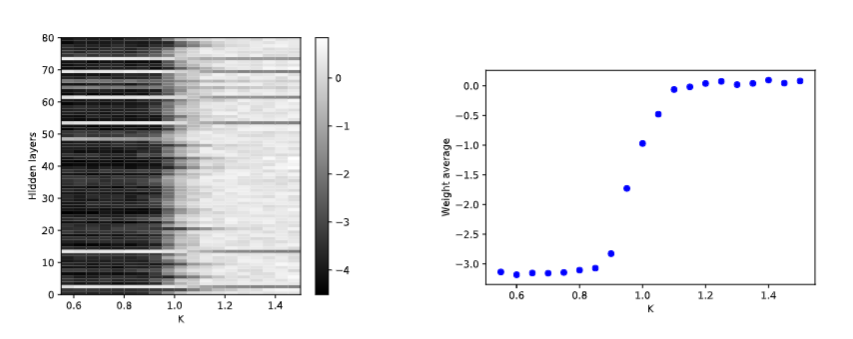
\includegraphics[height=5cm]{image/Figure2.png}
    \caption{2次元3状態ポッツ模型における学習後の全結合層での重みの値とそれらを平均した値.横軸はそれぞれ入力配位の温度$K$を表している.縦軸は左の図はニューラルネットワークの隠れ層につながるエッジにおける重みの値に対応し,右の図はその重みの値を$K$での平均をとったものである.重みの平均の値は,厳密な臨界温度$K_{\text{c}}^{\text{exact}}\simeq 1.0050$付近で大きく変化していることが見て取れる.}
  \end{center}
\end{figure}
2次元イジング模型の臨界温度の学習メカニズムの詳細に入る前に,別の例として2次元3状態ポッツモデルを見ていく.ハミルトニアンは以下のように表される.
\begin{equation}
  H(\{\Phi_i\}) = - \sum_{\langle i,j \rangle} \delta(\Phi_i, \Phi_j)
\end{equation}
ここで,$\Phi_i$は三つの値を取り,これはIsingスピン$\sigma_i$の一般化である.したがって,温度$K$でラベル付けされた配位$\{ \Phi_i \}$がニューラルネットワークの入力である.2次元3状態ポッツモデルは,単純なランダウ理論とは異なり,ゆらぎの影響で$K_c \approx 1.0050$で2次の位相転移を示すことが知られている[29-31].

\section{DISCUSSION}
これまでに,第二層の重みの値の変化が位相転移を示していることを観察してきた.これは,臨界温度の情報がなんらかの形で学習されたニューラルネットワークにコード化されていることを示唆している.以下では,学習された全結合型/畳み込み型のニューラルネットワークを注意深く検証し,それらが入力配位の特徴として抽出する(物理的な)量が何であり,それが温度の予測や臨界温度の検出とどのように関連しているかを理解しようとする[15, 17].

\subsection{ニューラルネットワークでエンコードされた磁化}
\begin{figure}[hb]
  \begin{center}
    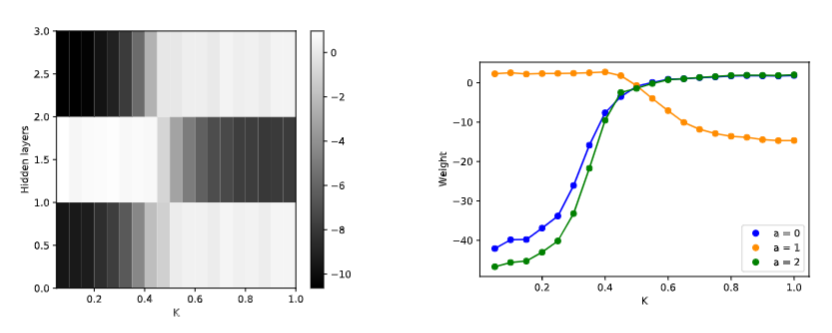
\includegraphics[height=5cm]{image/Figure3.png}
    \caption{隠れ層のユニットが3つ$(N_h=3)$の学習済みニューラルネットワークにおける全結合層の重み$w_{Ka}^{(2)}$の値.横軸は2次元イジング模型での温度$K$を表している.臨界温度付近で構造に変化が起きていることがわかる.真ん中の重みだけ値が反対になっている.}
  \end{center}
\end{figure}
\begin{figure}[hb]
  \begin{center}
    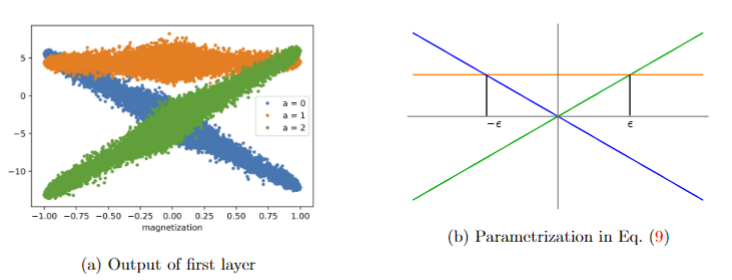
\includegraphics[height=5cm]{image/Figure4.png}
    \caption{(a)第1層目の出力と入力配位の磁化の相関.横軸は入力配位の各サイトでの磁化,縦軸は$\tilde{x}_a=w_{ai}^{(1)}\sigma_i+b_a^{(1)}$である.(b)フィッティングしたもの.}
  \end{center}
\end{figure}
相転移の秩序変数が2D Ising模型において自発磁化であることから,学習後にはその情報がニューラルネットワークにエンコードされていることは自然なことと言える.定量的な論拠を示すために,2D Ising模型の場合において学習されたニューラルネットワークの重みとバイアスを調査して,簡略化されたモデルを構築する.最初に、簡略化のために(2)の中の隠れユニットの数を80から3に減少させる.図3に示されているように,それでも臨界温度を捉えていることに気づく.\par
第二層をモデリングする前に,まず最初の層の特性を調査する.図4は,式(3)の第一層の出力$\tilde{x}_a \equiv w_{ai}^{(1)}\sigma_i + b_a^{(1)}$と,入力のIsingスピン配位の磁化密度との相関を示している.この観察から,私たちはこれらの出力から,図4bに示すように,磁化$m(\{ \sigma \})$に対して線形な三つのラインでモデリングする.
\begin{equation}
  \tilde{x} =
  \begin{pmatrix}
    \tilde{x}_0 \\ \tilde{x}_1 \\ \tilde{x}_2
  \end{pmatrix}
  =
  \begin{pmatrix}
    -m \\ \epsilon \\ m
  \end{pmatrix}
\end{equation}
ここで,$\epsilon > 0$は定数である.さらに,活性化関数として,私たちの目的のためにsoftmaxの代わりに最大値を1,それ以外を0にする最大値関数を使用している.この変更は最終結果に影響を与えない.$x_a = \max{(\tilde{x}_a)}$は次のベクトルを生成する.
\begin{equation}
  m<-\epsilon : x=
  \begin{pmatrix}
    1 \\ 0 \\ 0
  \end{pmatrix}, \
  -\epsilon \leq m < \epsilon : x=
  \begin{pmatrix}
    0 \\ 1 \\ 0
  \end{pmatrix}, \
  \epsilon \leq m : x=
  \begin{pmatrix}
    0 \\ 0 \\ 1
  \end{pmatrix},
\end{equation}
パラメータ$\epsilon$は、強磁性相と常磁性相を分離する閾値磁化と解釈できる[3].\par
三つの隠れユニットの磁化依存性を理解したら,次に第二層を分析する.この層の重みは図3に示されている.温度を低温,臨界温度,高温の三つの部分に分割する.それぞれ以下のベクトルで表される.
\begin{equation}
  \text{Low} \ \text{K} :
  \begin{pmatrix}
    1 \\ 0 \\ 0
  \end{pmatrix}, \
  \text{Critical} \ \text{K} :
  \begin{pmatrix}
    0 \\ 1 \\ 0
  \end{pmatrix}, \
  \text{High} \ \text{K} :
  \begin{pmatrix}
    0 \\ 0 \\ 1
  \end{pmatrix},
\end{equation}
No-dimensional output spaceにおいて.この手法により,出力次元$N_o$を実質的に3に削減する.図3に従って,私たちは以下のように重みをパラメータ化する.
\begin{equation}
  w^{(2)} =
  \begin{pmatrix}
    -\Delta & 0       & -\Delta \\
    -\delta & -\delta & -\delta \\
    0       & -\Delta & 0
  \end{pmatrix}
\end{equation}
ここで,$\Delta > \delta > 0$.行列$w^{(2)}$の$Ka$成分は$w_{Ka}^{(2)}$に対応する.バイアスは重みよりもはるかに小さいため,無視する.厳密なパラメータ化は,以下の議論には必要ない.このとき,$y_K = \max{(\tilde{y}_K)}=\max{(w_{Ka}^{(2)}x_a+b_K^{(2)})}$は以下の出力を生む.
\begin{align}
  m<-\epsilon : y_K = \max(w_{K0}^{(2)}) =
  \begin{pmatrix}
    0 \\ 0 \\ 1
  \end{pmatrix}, \\
  -\epsilon \leq m < \epsilon : y_K = \max(w_{K1}^{(2)}) =
  \begin{pmatrix}
    1 \\ 0 \\ 0
  \end{pmatrix}, \\
  \epsilon \leq m : y_K = \max(w_{K2}^{(2)}) =
  \begin{pmatrix}
    0 \\ 0 \\ 1
  \end{pmatrix},
\end{align}
これらはそれぞれ,低温,高温,低温と予想される.$m<-\epsilon$と$m>\epsilon$のスピン配位は秩序相にあるため,正しく予想できている.また,$-\epsilon \leq m < \epsilon$もまた,正しく予想されている.ただし,この場合には中間温度,つまり臨界温度を検出することができない.さらに,式(\ref{}) に三つ以上の対象温度を導入しても,学習されたニューラルネットワークは順序/無秩序相内の異なる温度を区別することができない.なぜなら,図3で示されているように,重み(およびバイアス)の上部ブランチはそれぞれ$K_c$より上と下でほぼ温度に依存しないからである.したがって,高温または低温のみを区別することができる.\par
これは,三つの隠れユニットにより単一の閾値パラメータ$\epsilon$しか持たないことが原因かもれない.隠れユニットをさらに導入することで閾値パラメータの数を増やすことができる.しかし,これは温度の高い精度にはつながらない.実際,隠れユニットの数を増やしても、,二層の重みは温度依存性の二つのパターンしか示さない.つまり,多くは図3の青と緑の曲線のようにふるまい,残りはオレンジの振舞いを見せる.これは,図1で観察されている現象とまさに一致している.隠れユニットを増やすことは単に,すでに図3で観察された第二層の重みを複製する結果となり,その結果,導入された隠れユニットの数に関係なく,予測される温度は高いか低いかのどちらかとなる.\par
上記の分析から得られた結論は次の通りである.
ネットワークは,第一層の出力で示す磁化の情報を取得した.しかしながら,ニューラルネットワークは磁化に基づいて秩序相と無秩序相の違いを除いて,温度を区別することは難しい.機械学習パラメータの観点から見ると,これは第二層の重みが臨界温度の周りを除いて温度に依存しないという事実に起因している.

\subsection{エネルギーと温度の予測}
前のサブセクションで,2次元イジング模型の磁化が温度の教師あり全結合ニューラルネットワークに組み込まれていることがわかった.これにより,その重み構造から臨界温度を読み取ることが可能になる.臨界温度はうまく検出されているようだが,温度そのものの予測自体についてはまだ議論していない.興味深いことに,2次元イジング模型の場合,上記の設定で温度学習の精度は理論的に$40.1\%$と計算できる.これは機械学習による温度予測の精度の上限を示しています([32].詳細は付録Aを参照).ただし、全結合ニューラルネットワークによる温度予測のテスト精度は$16.8\%$であり,理論的に予測された$40.1\%$の精度にはほど遠い.これまで,磁化の特徴抽出による相転移の検出を見てきたが,温度測定の観点で学習を行うことでより良い学習ができるのではないか.温度の予測精度が向上するようなニューラルネットワークを構築できた場合,どのようなことが起こるのか?\par
この疑問に答えるために,次に示す畳み込みニューラルネットワークを使用して,より高い精度を実現した.
\begin{equation}
  \begin{bmatrix}
    \begin{aligned}
       & \mathcal{I} = \left\{ \{ \sigma_i \} \Big| \ \text{Ising configs on} \ L \times L \ \text{lattice.} \right\}        \\
       & \downarrow
      \begin{cases}
        \text{Convolution}_{[(s_1,s_1)\text{-filter}, \ (s_1,s_1)\text{-stride}, \ C_1\text{-channels}]} \\
        \text{ReLU activation}                                                                           \\
        \text{Convolution}_{[(s_2,s_2)\text{-filter}, \ (s_2,s_2)\text{-stride}, \ C_2\text{-channels}]} \\
        \text{ReLU activation}                                                                           \\
        \text{Convolution}_{[(s_3,s_3)\text{-filter}, \ (s_3,s_3)\text{-stride}, \ C_3\text{-channels}]} \\
        \text{ReLU activation}                                                                           \\
        \text{Flatten}
      \end{cases} \\
       & x_a \in [0,1]^{N_h = L^2/(s_1s_2s_3)^2 \times C_3} \ \text{: hidden units}                                          \\
       & \downarrow
      \begin{cases}
        \text{Fully-connected (Dense) layer} \\
        \text{Softmax activation}
      \end{cases}                                                                                   \\
       & y_{\alpha} \in [0,1]^{N_t} \ \text{: output}
    \end{aligned}
  \end{bmatrix}
\end{equation} \label{conv model}
このネットワークは,3つの畳み込み層から配位されている.それぞれフィルタサイズ$(s_i,s_i)$,ストライド$(s_i,s_i)$,そして,チャンネル数$C_i$であり,それらの間にはReLU関数が入る.その後,出力は全結合層に渡される.この層の入力と出力は私たち興味の対象であり,詳細に分析される.第二最終層の出力,記号で$x_a$と示されるものは,以下のように表される.
\begin{equation}
  x_a = \text{ReLU}(\tilde{x}_a) = \text{Max}(\tilde{x}_a,0)
\end{equation}
これは$[0,\infty)$の範囲の値をとる.$\tilde{x}_a$は前の層のReLU関数の渡す前の出力である.その後、出力$x_a$は全結合層の入力として機能し,式(4)と(5)を通じて温度の予測を行う.\par
前のサブセクションに続き,私たちは,全結合層の入力として機能する3つの隠れユニットを配置し,学習の結果としてニューラルネットワークが何を学習するかを理解しようとする.この目的のために,パラメータは以下のように設定する:
\begin{equation}
  L = 16, \ \ (s_1, s_2, s_3) = (2, 2, 4), \ \ (C_1, C_2, C_3) = (64, 32, 3)
\end{equation}
これにより,隠れ層のユニット数を$N_{\text{h}}=3$にすることができる.このセットアップでは,テストデータセットにたいして$35.9\%$の精度を出すことができた.これは全結合層よりも2倍高いが,統計の不足と非常に少ない隠れユニット数のため,まだ境界に非常に近いわけではない.\par
\begin{figure}[ht]
  \begin{center}
    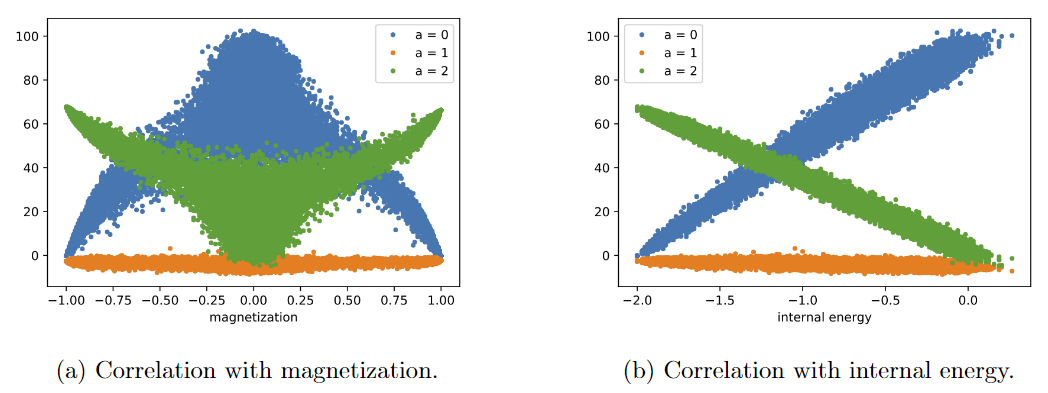
\includegraphics[height=5cm]{image/Figure5.png}
    \caption{学習されたニューラルネットワークの全結合層の重みと物理量との相関を示すもので,それぞれが左パネルおよび右パネルの垂直軸に対応する5つの隠れユニットがある.(a) および (b) の水平軸は,それぞれ2D Ising 配位の磁化および内部エネルギーを示す.\label{correlation}}
  \end{center}
\end{figure}
図\ref{correlation}は,第1層の出力と磁化(図\ref{correlation}a)および内部エネルギー(図\ref{correlation}b)との相関を示している.はっきりとニューラルネットワークが学習した内容の変遷が見て取れる.第1層の出力は,今では入力配位の磁化よりももしろ内部エネルギーに比例している.また,第2層の重みは温度に対して穏やかな依存性を示しており,臨界温度の情報がぼやけていることに気付く(図7);すぐに見るように,振動するオレンジの線は温度の予測には関係ない.\par
次は,最後の2層の簡略なパラメータ設定に進む.ここで,$(w_{ai}^{(1)}, b_a^{(1)})$および$(w_{ai}^{(2)}, b_a^{(2)})$はそれぞれ,最後から2番目の層および最後の層の重みとバイアスを表す.すでに述べたように,および図\ref{correlation}bで確認したように,第1層の出力は入力配位$\{ \sigma_i \}$のエネルギー$E(\{ \sigma_i \})$に比例している.ReLU関数を通ると,
\begin{equation}
  x_a = \text{ReLU}(w_{ai}^{(1)}\sigma_i + b_a^{(1)}), \ \
  x = \begin{pmatrix} x_0 \\ x_1 \\ x_2 \end{pmatrix}
  = \begin{pmatrix} E+2\epsilon \\ 0 \\ -\phi E \end{pmatrix}
\end{equation}
ここで,$\epsilon$と$\phi$は正の定数である.$E$の定義域は、$x_a$が負の値を取らないように制限されている.\par
全結合層の入力が$E$に比例していることを観察したので,入力配位 $\{\sigma_i\}$の温度の最適な推定が何であるかを考えてみよう.配位$\{ \sigma_i \}$が温度$K$で現れる確率$P(\{ \sigma_i \} ; K )$は
\begin{equation}
  P(\{ \sigma_i \} ; K )
  = \frac{e^{-KE(\{ \sigma_i \})}}{Z(K)}
  = e^{-KE(\{ \sigma_i \}) - \ln{Z(K)}}
  = e^{-KE(\{ \sigma_i \}) + F(K)}
\end{equation}
と表せされる.したがって,${\sigma_i}$ が温度$K$で生成される尤度は,
次の「確率」で表される.
\begin{equation}
  y_K^{\text{theory}} = \frac{P(\{\sigma_i ; K \})}{\sum_{K'}P(\{\sigma_i ; K' \})} = \text{softmax}(-KE + F)
\end{equation}
ここで,$F = -\ln{Z(K)}$は自由エネルギーで$K'$はすべてのターゲット温度での足し上げを意味する.このとき,私たちが得る推定温度は
\begin{equation}
  K^{\text{output}} =
  \underset{K} {\operatorname{argmax}} \left[\text{softmax}(-KE + F)\right]
\end{equation}
となる.ここで注記するのは,自由エネルギーが温度$K$の関数であり,有限な系では真の特異性を示さないものの,相転移の情報を保持しているということである.\par
上記の考察に基づいて,私たちのニューラルネットワークの全結合の重みを,その結果の出力が(21)のように振る舞うように推測する.その後,学習されたネットワークの実際のパラメータと比較する,このために,重みを以下のようにパラメータ化する.
\begin{equation}
  w_{K0}^{(2)} = -\phi G(K) - pK + q, \ \
  w_{K2}^{(2)} = -G(K) + rK + s
\end{equation}
定数パラメータ$p,q,r,s$および共通の非線形関数$G(K)$を持つようにする.図7のオレンジの曲線,$w^{(2)}_{K1}$は,$x_1 = \text{ReLU}(\tilde{x}_1) = 0$となるため,私たちの考慮には関係ない.バイアスの値が重みの値よりもはるかに小さい場合,バイアスを無視するというシミュレーションからの観察を利用している.\par
それでは,$y_K = \text{softmax}(w_{Ka}^{(2)}x_a + b_K^{(2)})$で式(19)と(23)を用いると,次のような出力が得られる.
\begin{equation}
  y_K = \text{softmax}(-(p+r)KE - 2\epsilon(\phi G(K) + pK))
\end{equation}
ここで,$\text{max}$関数に影響を与えないため,$K$に依存しない項は落とした.この式は,実際に$-2\epsilon (\phi G(K) + pK) = (p + r)F$が満たされる場合,$y_K^{\text{theory}}$の形をとる.理論的に予測された重みを図6にプロットした.
\begin{equation}
  w_{K0}^{(2)} = \frac{p+r}{2\epsilon}F(K) + q, \ \
  w_{K2}^{(2)} = \frac{p+r}{2\epsilon \phi}F(K) + \left( \frac{p}{\phi} + r \right)K + s
\end{equation}
\begin{figure}
  \begin{center}
    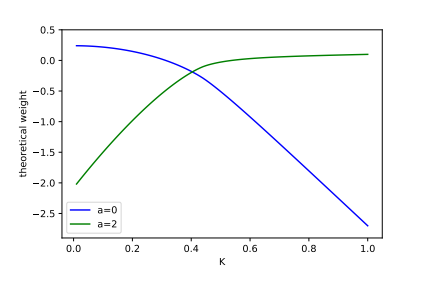
\includegraphics[height=4cm]{image/Figure6.png}
    \caption{青,緑の線はそれぞれ式(23)の$w_{K0}^{(2)}$と$w_{K2}^{(2)}$を表している.水平軸は,入力の2D Ising配位の温度Kを表している.詳細は本文を参照.}
  \end{center}
\end{figure}
\begin{figure}
  \begin{center}
    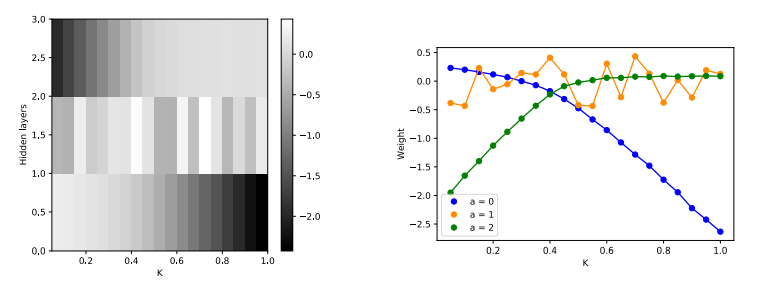
\includegraphics[height=4cm]{image/Figure7.png}
    \caption{3つの隠れユニット$H_{\text{h}}=3$を持つ学習された畳み込みニューラルネットワークの全結合の重み.水平軸は,入力の2次元Ising模型の温度$K$を表している.最初と最後の重みの値は,以前のケースとは対照的に,温度が上昇するにつれて徐々に変化する.詳細な議論については本文を参照.}
  \end{center}
\end{figure}
$F(K)$は2次元Ising模型で解析的に計算された自由エネルギーである.これは,図7に示される学習されたニューラルネットワークから得られた実際の重みと非常によく一致している(青と緑の曲線).これらの考察に基づいて,相転移の情報は再び全結合の重みに符号化されていると結論する.なぜなら,式(23)の$G(K)$は直接的に自由エネルギーと関連しているからである.特に,臨界温度は,温度に関する重みの2階導関数の増加を検出することによって得られる.\par
上記で示したモデルや重みのパラメータ設定は,同じ温度予測を生じる多くの可能性のうちの一つであることに注意してほしい.たとえば.2次の$K$依存性は,重みではなく最後の層のバイアスから生じる可能性がある[32].その場合,相転移や自由エネルギーの情報はバイアスに符号化されるはずである.物理的な情報が機械のパラメータにどのように格納されるかは、隠れユニットの数や活性化関数などを含むニューラルネットワークのアーキテクチャに依存する\par
ニューラルネットワークの内部構造に対する洞察を得たことから,物理的な観点から畳み込みニューラルネットワークが完全に接続された層だけから成るネットワークよりも温度をより正確に予測できる理由について論じる.このセクションで観察したように,後者は中間層で磁化を捉えるが,前者は内部エネルギーを抽出し,それに基づいて温度を推測しようとする.ただし,Ising模型における磁化の温度依存性は,臨界温度周辺以外では内部エネルギーと比較して小さい.したがって,ニューラルネットワークがより正確な温度予測のために内部エネルギーの情報を抽出するのは妥当である.実際,畳み込みニューラルネットワークは内部エネルギーを成功裏に学習して,より高い精度を実現している.畳み込みニューラルネットワークの方が優れたパフォーマンスを発揮する理由は,畳み込み層がIsingスピンの空間的な相関などの空間構造を利用して,入力スピン構造の特徴を識別する能力があるためである.一方で,全結合層はその構造には無視されます.最後に,2次元Ising模型に対して与えられた議論は,3状態ポッツモデルにも当てはまることを触れておく.\par

\section{結論}
私たちは,温度による教師あり機械学習を用いて2次元Ising模型の相転移検出を再検証し,その基本的なメカニズムを明らかにした.\par
まず,全結合ニューラルネットワークが2次元Ising模型および3状態ポッツ模型の学習の結果として,第2層の重み構造に急激な変化を示すことを示した.3つの隠れユニットを持つニューラルネットワークを詳しく調べると,実際には第1層で磁化を捉えていることが明らかになった.相転移の検出は,臨界温度周辺以外の入力配位に対する温度の低い予測精度の結果である.\par
一方で,畳み込みニューラルネットワークを使用することで,温度予測の精度を向上させることに成功した.学習された畳み込みネットワークは,磁化ではなく入力配位の内部エネルギーを捉えていることが判明した.また,最後の全結合層の重みは,前者のケースとは対照的に値に急激な変化を示さず,これは最適な温度予測の観点から理解できます.この場合,重みは自由エネルギーに比例しており,したがって,臨界温度を含む物理的な情報が再びこれに符号化されている.\par
興味深いことに,学習されたニューラルネットワークは,どのように学習されたかによって異なる物理的な情報を抽出する.温度予測の観点から見て「悪い」ニューラルネットワークは,入力スピン構造の磁化を捉えようとしますが,これは臨界温度を検出するのに便利であることがある(これは秩序変数であるため).ネットワークアーキテクチャの改善により,「良い(より良い)」温度予測器を構築することができる.ただし,相転移の情報はネットワークにより暗黙的に符号化される.

\subsection*{Appendix A : 温度測定器と精度}
イジングスピン配位の温度予測がどのように機能するかを考える[32].まず,目標温度でのマルコフ連鎖モンテカルロアルゴリズムによって生成されたイジングスピン配位を用意する.ある固定された温度$K$における配位は,エネルギーにわたって分布しており,その平均$\langle E \rangle$と分散$\langle E^2 \rangle - \langle E \rangle^2$は次のように与えられる.\par
\begin{equation}
  \langle E \rangle = \frac{\sum_{\{ \sigma_i \}}H(\{ \sigma_i \})e^{-KH(\{ \sigma_i \})}}{\sum_{\{ \sigma_i \}}e^{-KH(\{ \sigma_i \})}}
\end{equation}
\begin{equation}
  \langle E^2 \rangle - \langle E \rangle^2
  = -\frac{\partial}{\partial K}\langle E \rangle
  = \frac{\partial^2}{\partial K^2} \ln{Z}
\end{equation}
スピン配位が与えられると,温度の最適な予測を考える.各配位のエネルギーは計算ができる.エネルギー密度$E/L^2$の標準偏差が$L^{-1}$に比例しているため,エネルギーの確率分布は無限系では幅を持たないことに注意しておこう.この場合,ある特定の配位が与えられた場合,そのエネルギー密度を計算することによって,それが生成された温度を正確に予測できるはずである.しかし,有限サイズの系を考慮すると,各温度での分布は有限の幅を持つ.その場合,エネルギー分布の重なりがあるため,温度予測が必ずしも正しい答えを与えるわけではない(図8).私たちができる最善のことは,最尤推定によって配位の温度を推測することである.つまり,配位のエネルギーを最も可能性が高くする温度が最適に予測された温度である.その結果,有限系でのエネルギー確率分布の重なりから,予測の精度には上限がある.\par
\begin{figure}
  \begin{center}
    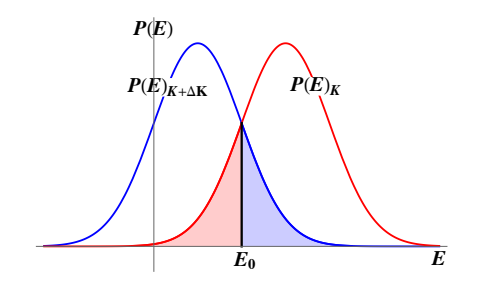
\includegraphics[height=4cm]{image/Figure8.png}
    \caption{2つの隣り合った温度$K$と$K+\Delta K$におけるエネルギー分布.分布が重なっている部分は赤と青の影付きの領域で示されている.赤い分布は温度$K$で生成される.ただし,赤い影付きの領域にある場合,最尤法ではこれらの配位は温度$T+\Delta T$のものとして誤分類される.($E_0$以下では$P(E)_{K+ \Delta K} > P(E)_K$).同じ議論で青い影付き領域で生成された配位にも当てはまる.}
  \end{center}
\end{figure}
2次元Ising模型を詳しく見ていこう.これは正確に解かれている[28]ので,自由エネルギー密度の明示的な表現がある.
\begin{equation}
  f = -\frac{\ln{Z}}{2} - \ln{[\cosh{2K}]} - \frac{1}{2\pi}\int_{0}^{\pi}d\theta \ \ln{\left[1 + \sqrt{1- \left(\frac{2\sinh{2K}}{\cosh^2{2K}}\cos{\theta}\right)^2}\right]}
\end{equation}
サイト数はNで,有限サイズ効果は考慮していない.次に,興味のある温度でのエネルギー確率分布を,平均が$\langle E \rangle$で分散が$\langle E^2 \rangle - \langle E \rangle^2$のガウス分布で近似する.図9に,20の異なる温度$K = 0.05, 0.1, 0.15, \dots, 1.0$におけるエネルギー分布を示した.
\begin{figure}
  \begin{center}
    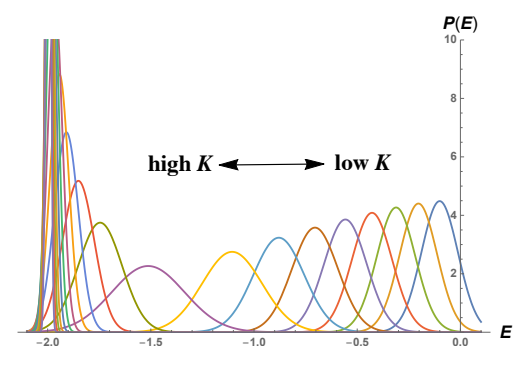
\includegraphics[height=4cm]{image/Figure9.png}
    \caption{2次元Ising模型における温度$K = 0.05, 0.1, 0.15, \dots, 1.0$におけるエネルギー確率分布.垂直軸はサイトあたりのエネルギーで,サイト数は$16\times 16$としている.}
  \end{center}
\end{figure}
分布間の重なりが大きいことがわかるが,臨界温度$K_{\text{c}}^{\text{exact}} \sim 0.4407 $の周りで減少している.最尤推定によって得られる精度は$40.1\%$に過ぎず、機械学習によって構築された温度計は最大で$40.1\%$の精度しか達成できないことを意味している.それにもかかわらず,学習されたニューラルネットワークは相転移検出器として機能することがわかる.





\end{document}